%-----------------------------------------------------------------------------------------------
\section{Performance comparison}
%-----------------------------------------------------------------------------------------------

The major part of this work is dedicated to selecting the most suitable algorithm for measuring quad parameters.
So far the theory of the underlying algorithms and the minimum viable implementations of detectors based on them have been discussed.
In order to select the best candidate some kind of benchmarking solution is needed.
Defining a scoring function to be used as a base for comparison was a task to be solved.
Also, to draw any meaningful conclusion a significantly large number of test need to be run.

To address these tasks, a test framework was developed.
Similarly to the detectors themselves, it was also done in python.
The software handles the whole benchmarking process.
It generates quads for test data, renders them to images, runs the detection routines, plots the test result, etc...
This test framework is described with the necessary level of detail in this section.

It was also a non-trivial decision to select a scoring function for the comparison.
Below will be a summary of the tried and used error functions.
The reasons for their consideration as well as their definitions will be explained.

The last, major part of this section will be the discussion of the test results.
Each algorithm will have a thorough analysis about it's strengths and weaknesses, and of their error distribution.
Finally, the summary of the results will be published, comparing the performance of the detectors.
Based on those results, an algorithm will be chosen as recommended for use.

%-----------------------------------------------------------------------------------------------
\subsection{Test method}
%-----------------------------------------------------------------------------------------------

In this project multiple quad detection solutions are prototyped.
The best is needed to be selected.
It is not a trivial choice, as there are many criteria to be satisfied.
The algorithm needs to be accurate, robust, relatively fast, work on noisy images, etc...
Thorough testing is necessary to select the best algorithm for the task.
The tests should be reproducible and statistically relevant.
In this section will be a description of the testing method used in this project.

As a first step, a data source is necessary for the algorithms under test.
For this, randomly generated quads were used.
The random generator was constructed in a way that allowed some control over the generated data: the \textit{quad size} and the range of the other parameters could be set.
To provide data for extensive testing, a large data set was generated.
Every algorithm received random quads with sizes ranging from $1\%$ to $75\%$ of the image size, in $1\%$ increments.
From each size 1000 quads were generated and provided to the detectors.
These values were chosen to cover a significant portion of the parameter space and to provide statistically significant results.

The generated quads were rendered by OpenCV and the generated images were the inputs for the detection algorithms.
The testing was done with images containing only a single quad.
There are many reasons for this.
First, it is important to limit the test scope.
In this step the quad detection was benchmarked. not the segmentation logic.
In the real use-case, the input image containing a marker is segmented, and the segments are fed to the quad detector separately.
The images were rendered with different levels of additive Gaussian White Noise.
The test series were run first on optimal images, and after that rerun with more and more added noise.
This was done to test the robustness.
Although the GWN covers only a small portion of the noise in a real image, these test did provide some insight.

The accuracy of the detection was analysed based on many different error measure.
Those are defined in the next section.
The experiments measured the expected value and the standard deviation of error of the algorithms.
These were plotted at the end of the test cycle.

The test method is summarised by the following pseudo-code program.
%test cycle in pseudo code
\begin{lstlisting}
quad_groups = empty_list
for size in [0.01:0.01:0.75]:
	group = generate_quads(count=1000, size=size)
	quad_groups.append(group)

error_series = empty_list
for group in quad_groups:
	pairs = empty_list
	for quad in group:
		img = render(quad)
		img = add_noise(img, noise_level)
		detected_quad = detector.detect_quad(img)
		pairs.append(quad, detected_quad)
	group_error = calculate_error(pairs)
	error_series.append(group_error)
display_result(error_series)	
\end{lstlisting}

The quads were rendered to $640*640$ \textit{pixel} images.
The quad sizes (base lengths) are normed to image size, that is $640 px$.
A quad with size 1 would have a 640 pixel long base.
The same scaling applies to the diagrams of the following sections. 

%-----------------------------------------------------------------------------------------------
\subsection{Error measure}
%-----------------------------------------------------------------------------------------------

In order to compare the performance of the quad detection algorithms some kind of scoring function is needed.
For this the use of detection error seems intuitive.
As a quad has 6 independent parameters, and these are stored in 2 different representations, defining an error measure is not straightforward.
Because of this, several scoring functions were defined during development, and many of those are actually used for comparing the algorithms.

As described in the previous section, the calculation of detection error is based on rendering a known quad and running the detection algorithms on it.
After the detection is done and it is successful\footnote{A quad instance is returned, which is not guaranteed}, some kind os measure is necessary to calculate the "distance" of the detected and the original quad.
Below will be the definitions the error measures used within this project to compare the quad detection algorithms.
The notations used in the formulae are listed here.
% notation
\begin{itemize}
	\item $Q^o, Q^d$: Original quad, detected quad
	\item $Q_p$: Parameter $p$ of quad $Q$, where $p$ can be any of the followings: $\{s, m_a, m_b, \alpha, \beta, \gamma\}$. 
	\item $C^o, C^d$: Corner set of the original and the detected quad
	\item $C_i^o, C_i^d$: The $i.$ corner of the original and the detected quad
	\item $C_{i,x}$: $x$ coordinate of the $i.$ corner of a quad
	\item $P^o, P^d$: the parameter space of the original and the detected quad. Using Section \sectref{quad}'s notation, it can be defined as $P = \{s, m_a, m_b, \alpha, \beta, \gamma\}$
\end{itemize}

As mentioned above, there are two different quad representations used\footnote{for details, see Section \sectref{quad}}.
One stores the coordinates of the corners, the other the quad parameters.
The most intuitive way for error calculation is based on the corner representation.
We can calculate the distance between the detected and the original corner.
\eqref{errAbsSumCoord}, \eqref{errAbsAvgCoord} and \eqref{errRelAvgCoord} define 3 scoring functions based on this idea. 
% sum of absolute position error
\begin{equation}
	E_{c,abs} = \sum_{1}^{4} \sqrt{(C_{i,x}^o - C_{i,x}^d)^2 + (C_{i,y}^o - C_{i,y}^d)^2}
	\label{eq:errAbsSumCoord}
\end{equation}
The first possibility is to calculate the sum of the distance between the detected and the original corners.
This naive approach has many drawbacks.
The main concern is that it does not take into account the \textit{size} of the quad.
The cumulation of error from every corner also distorts the results.
In reality, if every corner has some amount of noise in it's position, the quad parameter representation can still be quite close to the original.
However, if only one corner has a larger amount of error, the distortion will be much higher.
This error measure reports the same amount for both cases.
% avg absolute position error
\begin{equation}
	E_{c,avg} = \frac{1}{4} E_{c,abs}
	\label{eq:errAbsAvgCoord}
\end{equation}
The above points are also true is the average of the absolute displacements are used.

Better results can be achieved by using relative coordinate error.
The formula used by this work can be seen in \eqref{errRelAvgCoord}.
The problem of the error depending on the quad \textit{size} is solved by this.
As seen on the formula, the coordinate error is compared to the coordinates of the original quad corners.
% avg relative position error
\begin{equation}
	E_{c,rel} = \frac{1}{4}\sum_{1}^{4} \frac{\sqrt{(C_{i,x}^o - C_{i,x}^d)^2 + (C_{i,y}^o - C_{i,y}^d)^2}}{\sqrt{(C_{i,x}^o)^2 + (C_{i,y}^o)^2}}
	\label{eq:errRelAvgCoord}
\end{equation}
\eqref{errRelAvgCoord} was chosen for the comparison of algorithms based on the accuracy of corners detected.

The following scoring functions are based on the other quad representation.
This has considerable advantages compared to the corner based representation, because a much clearer picture of the distribution of error factors is obtained.
The quad parameters can be classified into 3 sets.
The is the quad size, which is an absolute length, measured in pixels.
Another category is formed of the angle parameters: the angle between the \textit{base} and each \textit{arm}, and the orientation (which is basically the angle between the \textit{base} and the image frame).
The third is the multiplier parameter.
These are not absolute lengths, they are calculated based on the base length.
Below will be proposed error measures for the three categories.

For the angle parameters, as a first approach an absolute error measure was defined.
As \eqref{errAbsSumAngle} shows, the 2 angle errors are summed.
As an alternative, their average also can be used.
Contrary to the coordinate errors, here the absolute angle error does not depend on the size of the quad.
These scoring functions can be useful if the absolute magnitude of the error is of interest.
% sum of absolute angle error
\begin{equation}
	E_{a,abs} = |Q_\alpha^o - Q_\alpha^d| + |Q_\beta^o - Q_\beta^d|
	\label{eq:errAbsSumAngle}
\end{equation}
% avg absolute angle error
\begin{equation}
	E_{a,avg} = \frac{1}{2} E_{a,abs}
	\label{eq:errAbsAvgAngle}
\end{equation}
Of course, relative error can also be defined for the angles, too.
See \eqref{errRelAvgAngle}.
This was used for comparison, because the relative values given as percentages were easier to evaluate.
% avg relative angle error
\begin{equation}
	E_{a,rel} = \frac{1}{2}\Bigg(\frac{|Q_\alpha^o - Q_\alpha^d|}{|Q_\alpha^o|} + \frac{|Q_\beta^o - Q_\beta^d|}{|Q_\beta^o|}\Bigg)
	\label{eq:errRelAvgAngle}
\end{equation}

The multipliers are very similar to the angles in terms of error metrics.
They describe a relative parameter, so the quad scale is not an issue here.
Nonetheless, both absolute and relative error measures were defined for completeness.
Similarly to the angles, both the sum os absolute errors and their average can be meaningful, depending on what is the goal of analysis.
% sum of absolute multiplier error
\begin{equation}
	E_{m,abs} = |Q_{ma}^o - Q_{ma}^d| + |Q_{mb}^o - Q_{mb}^d|
	\label{eq:errAbsSumMul}
\end{equation}
% avg absolute multiplier error
\begin{equation}
	E_{m,avg} = \frac{1}{2} E_{m,abs}
	\label{eq:errAbsAvgMul}
\end{equation}
For readability, the relative measure was chosen as a basis for comparison.
The values are normed with the respective parameter of the original (generated, thus it's parameters are known to an arbitrary level of precision) quad.
% avg relative multiplier error
\begin{equation}
	E_{m,rel} = \frac{1}{2}\Bigg(\frac{|Q_{ma}^o - Q_{ma}^d|}{|Q_{ma}^o|} + \frac{|Q_{mb}^o - Q_{mb}^d|}{|Q_{mb}^o|}\Bigg)
	\label{eq:errRelAvgMul}
\end{equation}

Orientation is handled differently from the other angle parameters.
This is due to two reasons.
First, it's conceptually different.
It describes a rotation as opposed to $\alpha$ and $\beta$ that describe angles between lines segments.
The second reason is mainly empirical: it turned out to be less error-prune than the other two.
% absolute orientation error
\begin{equation}
	E_{o,abs} = |Q_\gamma^o - Q_\gamma^d|
	\label{eq:errAbsOrient}
\end{equation}
% relative orientation error
\begin{equation}
	E_{o,rel} = \frac{|Q_\gamma^o - Q_\gamma^d|}{|Q_\gamma^o|}
	\label{eq:errRelOrient}
\end{equation}
Similarly to the previously discussed categories, the absolute and relative errors are defined.
Equations \eqref{errAbsOrient} and \eqref{errRelOrient} show the definitions.
For comparison, as before, the relative error was used.

The \textit{base length} or \textit{size} is the only absolute length parameter in this quad representation.
It makes sense to handle it separately, because many other parameters (orientation, arm multipliers) depend on it.
The scoring functions are defined below, similarly to the previous ones.
% absolute size error
\begin{equation}
	E_{o,abs} = |Q_s^o - Q_s^d|
	\label{eq:errAbsSize}
\end{equation}
% relative size error
\begin{equation}
	E_{o,rel} = \frac{|Q_s^o - Q_s^d|}{|Q_s^o|}
	\label{eq:errRelSize}
\end{equation}
For consistencies sake, also the relative error was used here for comparison.

The above defined error functions provide useful information if the distribution of error between the quad parameters is interesting.
However, this parametric quad representation lacks a scoring function that would provide information on the error magnitude as a whole.
To resolve this, one more error measure is proposed and used by this work.
The independent parameters of a quad can be viewed as coordinates in a 6 dimensional space.
The analogy stands, as the parameter space is a subset of $\mathbb{R}^6$.
A distance in that 6-dimensional space can be defined, see \eqref{errQuadSpaceDist}.
% distance in parameter space
\begin{equation}
	E_{sum} = \sqrt{\sum_{p \in P^o, q \in P^d} (p - q)^2}
	\label{eq:errQuadSpaceDist}
\end{equation}
This gives useful information about the absolute magnitude of error in the parametric quad representation.
Of course, the relative version of the above error measure can also be defined.
% distance in parameter space, relative
\begin{equation}
E_{sum, rel} = \frac{\sqrt{\sum_{p \in P^o, q \in P^d} (p - q)^2}}{\sqrt{\sum_{p \in P^o} p^2}}
\label{eq:errQuadSpaceDistRel}
\end{equation}
With this, a complete set of error measurement functions are defined.

It is reasonable to use both quad representations, thus both sets of error measures.
The corner representation is intuitive.
Also, as it is stated in the previous chapters of this work, the pose estimation algorithms use corresponding point pairs.
So the most relevant error component seems to be the one present in the quad corner coordinates, as it directly influences the accuracy of the calculated camera pose.

However, the two representations are equivalent.
It is possible to convert between the two without loosing useful information.
If discrete markers are used, with the parametric representation it is possible to further refine the detection results.
This can be done by replacing the detected quad with the closest known discrete one\footnote{This will be elaborated later on. This sentence is just to give a general idea and is not technically correct.}.
Currently this aspect of the marker is not implemented, it can be a subject of future improvements.

%-----------------------------------------------------------------------------------------------
\subsection{LSD Quad Detector results}
%-----------------------------------------------------------------------------------------------

\begin{figure}[t]
	\centering
	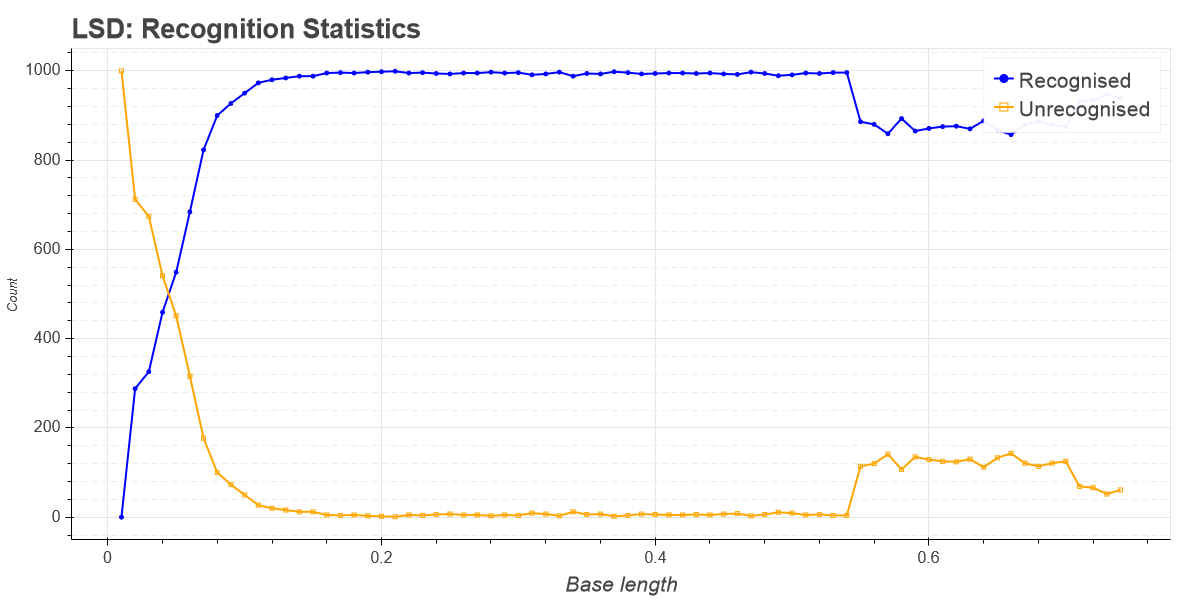
\includegraphics[width=0.9\textwidth]{figures/plots/lsd_rec_unrec_count.png}
	\caption{Recognised and unrecognised quads with respect to quad size, using the LSD method}
	\label{fig:lsdRecCnt}
\end{figure}
In this section the performance of the Line Segment Detector-based quad detection method will be evaluated.
Figure \figref{lsdRecCnt} shows the recognition count of the LSD quad detector.
Recognition fail is reported by the test framework if the detector couldn't find a quad on the input image or the average relative error is greater than $100\%$.
Detection failure can be caused by a couple of reasons within the algorithm.
If the quad on the image is too small, less than 3 lines may be detected.
The detector is helpless in this case, no quad is returned.
Another failure cause is connected to the small quads.
\begin{figure}[ht]
	\centering
	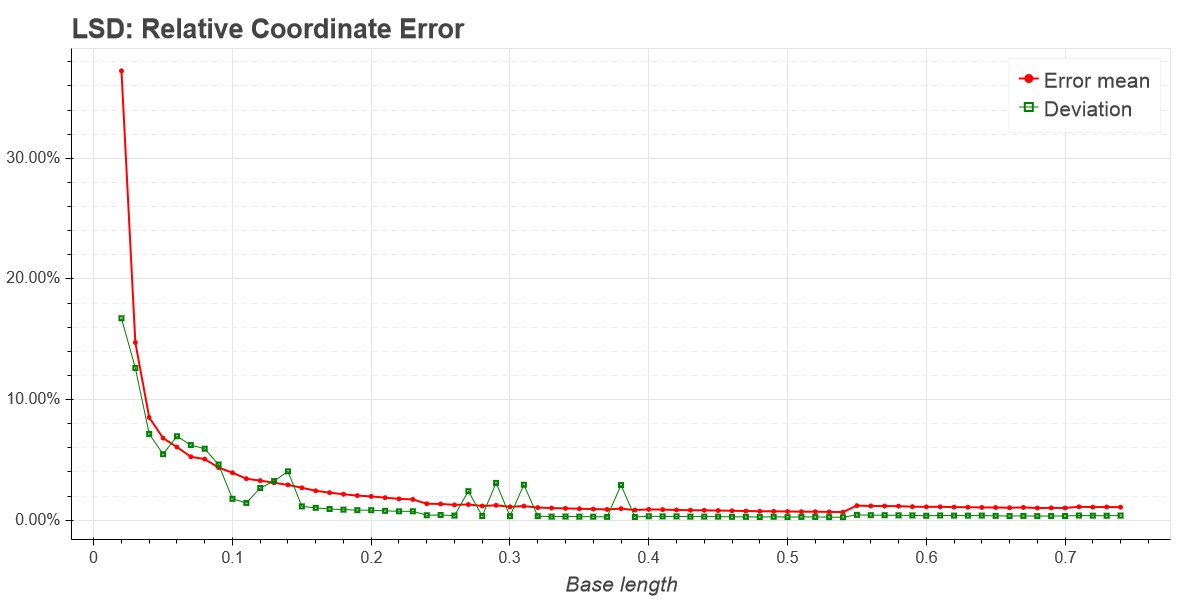
\includegraphics[width=0.9\textwidth]{figures/plots/lsd_relative_coordinate_error.png}
	\caption{Relative coordinate error with respect to quad size, using the LSD method}
	\label{fig:lsdRelCoordErr}
\end{figure}
If the necessary number of line segments are detected, it is still possible for the detection to fail.
It can happen because a small quad rendered in comparatively low resolution looks more like a blob than connected line segments, thus the detected segments are not necessarily correspond to the segments of a quad.
These effects combined explain the rising edge in the beginning of the detected quad count on figure \figref{lsdRecCnt}.

\begin{figure}[ht]
	\centering
	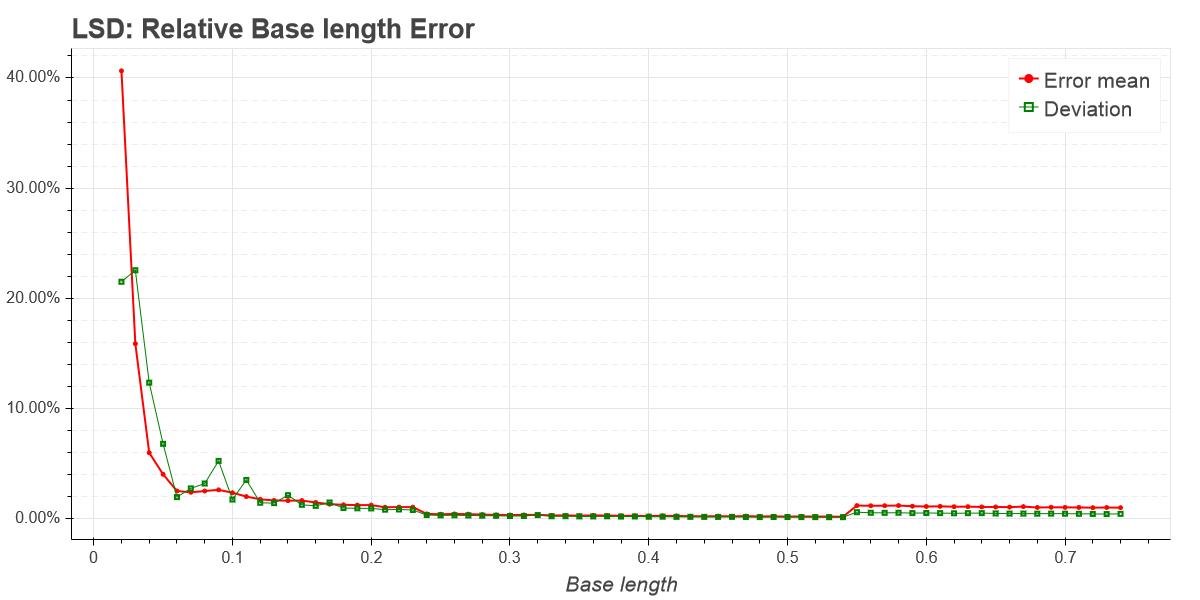
\includegraphics[width=0.9\textwidth]{figures/plots/lsd_relative_base_length_error.png}
	\caption{Relative base length error with respect to quad size, using the LSD method}
	\label{fig:lsdRelBaseErr}
\end{figure}
The sudden increase in the unrecognised count in the region of larger quads can be caused by a combination of two effects.
The quad rendering process is designed in a way that larger quads are rendered with thicker lines than the small ones.
This can cause issues with the merging of the two edges into one line.
The detector algorithm can be improved to better handle this.
The other part is that the LSD algorithm is sensitive to the scale of the features compared to the image size.
Detection can be improved if the algorithm is re-run on a down-sampled image.

\begin{figure}[ht]
	\centering
	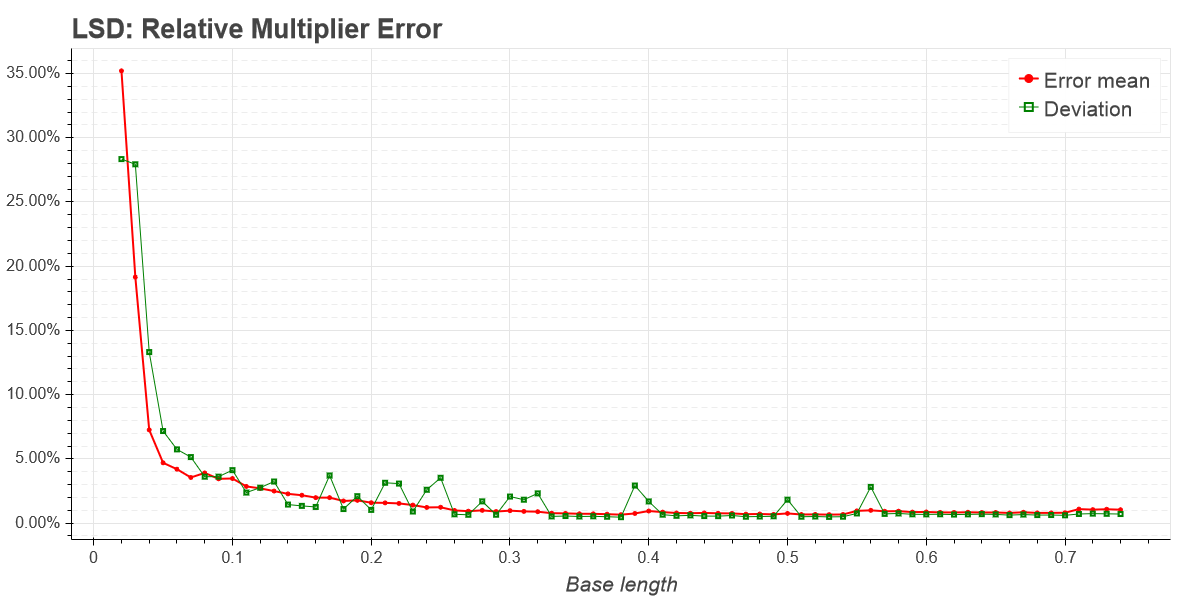
\includegraphics[width=0.9\textwidth]{figures/plots/lsd_relative_multiplier_error.png}
	\caption{Relative multiplier error with respect to quad size, using the LSD method}
	\label{fig:lsdRelMulErr}
\end{figure}
The overall performance of the LSD quad detector is quite good.
Figure \figref{lsdRelCoordErr} shows the average relative coordinate error and it's deviation as a function of the quad size.
This figure can be used as an indicator of the general performance the algorithm.
The relative coordinate error is below $5\%$ before the 0.1 scale factor is reached.
This means that the algorithm can detect quite small features relatively accurately.
In the optimal case, the average error is below $1\%$.
As the figure shows, the deviation of the error is also small, which indicates that the detection is stable.

\begin{figure}[ht]
	\centering
	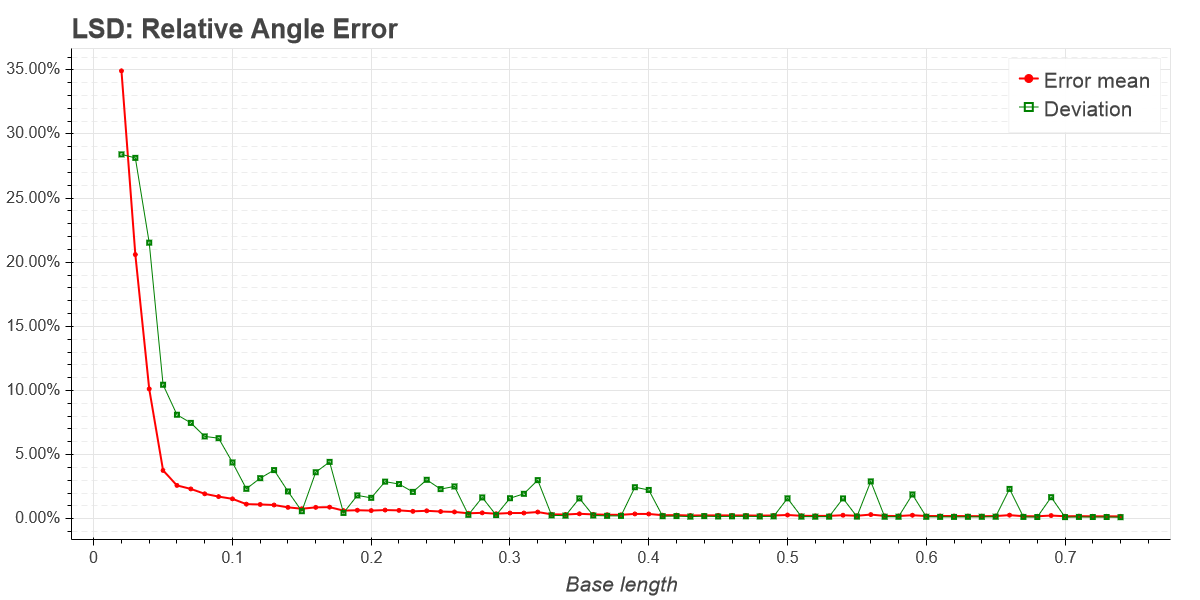
\includegraphics[width=0.9\textwidth]{figures/plots/lsd_relative_angle_error.png}
	\caption{Relative angle error with respect to quad size, using the LSD method}
	\label{fig:lsdRelAngleErr}
\end{figure}
The rest of the quad parameters show roughly the same level of accuracy.
The angle error (figure \figref{lsdRelAngleErr}) and the multiplier error (figure \figref{lsdRelMulErr}) stay below $5\%$ for most of the usable size range.

The error in the detected coordinates, base length, and multipliers show a small increase toward the region of larger quads.
This is caused by the same effect as causes the increase in recognition failure.
However, the angle parameters are not affected by this issue.
This is not unexpected, as the angle between lines is left unchanged by the offset caused by the line width. 

Another interesting observation can be made about the error distribution.
Figure \figref{lsdRelBaseErr} and \figref{lsdRelOrientErr} show a significantly smaller error level than the others.
Both the base length and the orientation only depends on the detection of the quad base, which is usually the largest feature of a quad.
This results in a more accurate detection, as more inliers are available for precise line detection.
The orientation is the most accurately detectable quad parameter. 
On top of it depending only on the quad base, it is unaffected by the error in the detection of the base length.
Only the angle of the line is important.
\begin{figure}[ht]
	\centering
	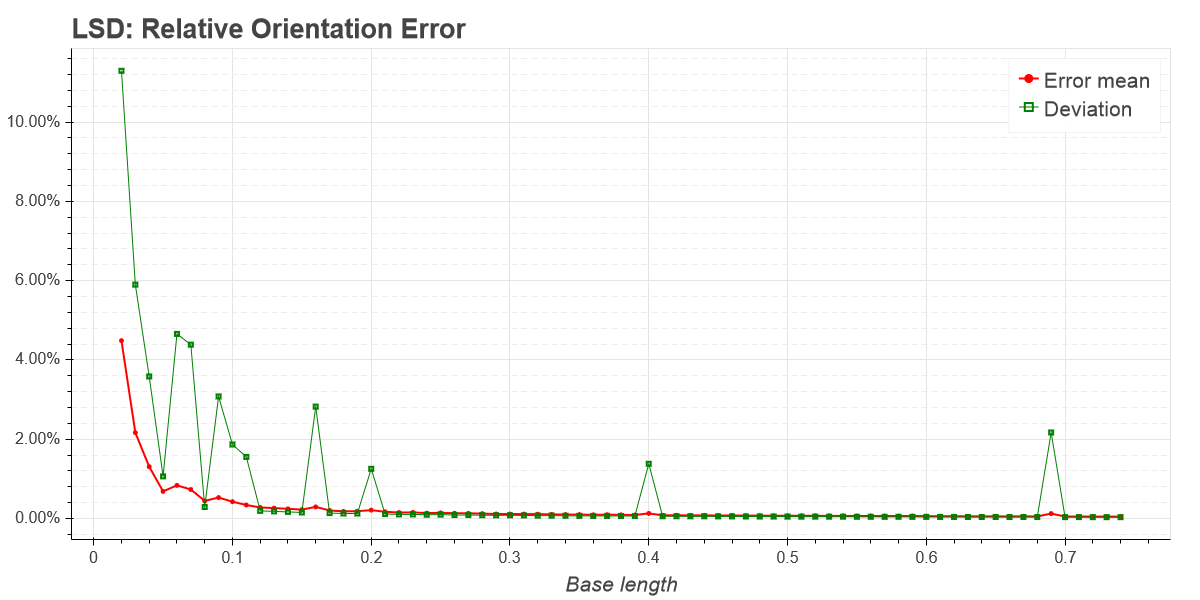
\includegraphics[width=0.9\textwidth]{figures/plots/lsd_relative_orientation_error.png}
	\caption{Relative orientation error with respect to quad size, using the LSD method}
	\label{fig:lsdRelOrientErr}
\end{figure}

Although the runtime of the algorithms was not measured during the experiments, the LSD method was noticeably faster than the others.
For any meaningful statistics on runtime, an equally well optimised, preferably C++ implementation of the algorithms would be necessary.
This was not in the scope of this project.

%-----------------------------------------------------------------------------------------------
\clearpage\subsection{SHT Quad Detector results}
%-----------------------------------------------------------------------------------------------

This quad detection method is built around the Standard Hough Transform, with all of it's well known benefits and drawbacks.
It provides usable results, but there are better alternatives amongst the tested detectors.
Below is the performance analysis of the SHT-based detector.

\begin{figure}[t]
	\centering
	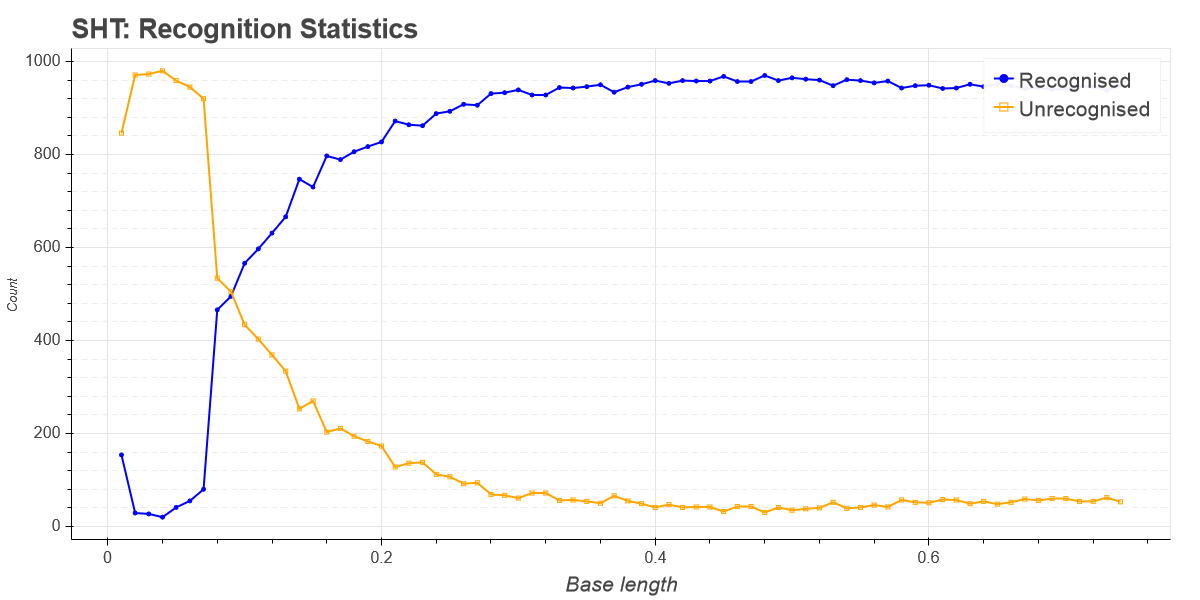
\includegraphics[width=0.9\textwidth]{figures/plots/sht_rec_unrec_count.png}
	\caption{Recognised and unrecognised quads with respect to quad size, using the SHT method}
	\label{fig:shtRecCnt}
\end{figure}

\begin{figure}[ht]
	\centering
	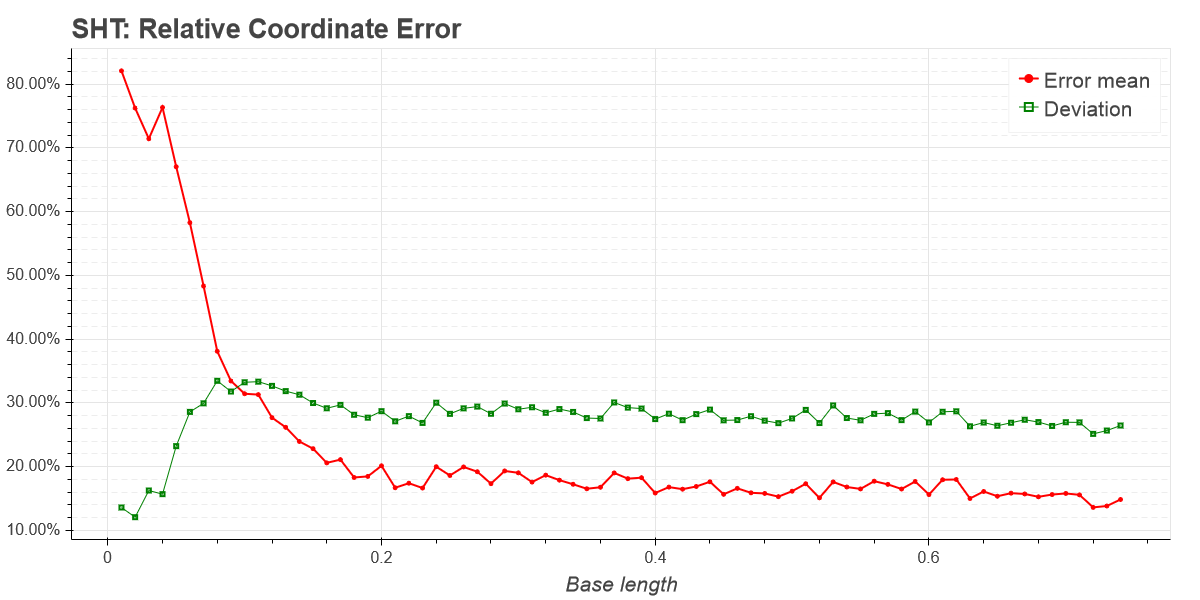
\includegraphics[width=0.9\textwidth]{figures/plots/sht_relative_coordinate_error.png}
	\caption{Relative coordinate error with respect to quad size, using the SHT method}
	\label{fig:shtRelCoordErr}
\end{figure}
Figure \figref{shtRecCnt} shows the recognition statistics of the detector.
It needs much larger quads to work, compared to the other detectors.
This is partly caused by the SHT's need to have a comparatively large number of inliers supporting a line to detect it.
For small quads, some line segments can be simply shorter than what is detectable by the algorithm.
Or false line can be detected, which also makes the quad reconstruction impossible.

The Hough transform has tunable parameters, which greatly affect what features can be found.
However, there is no formula to determine the values of these optimally based on the image parameters, so some heuristics are necessary to guess them.
The detection rate could possibly be optimised by tweaking that heuristics, but it is outside the scope of this project.
For now, it is accepted as a limitation that the SHT-based quad detector provides useful information above the $0.2$ quad size.
\begin{figure}[ht]
	\centering
	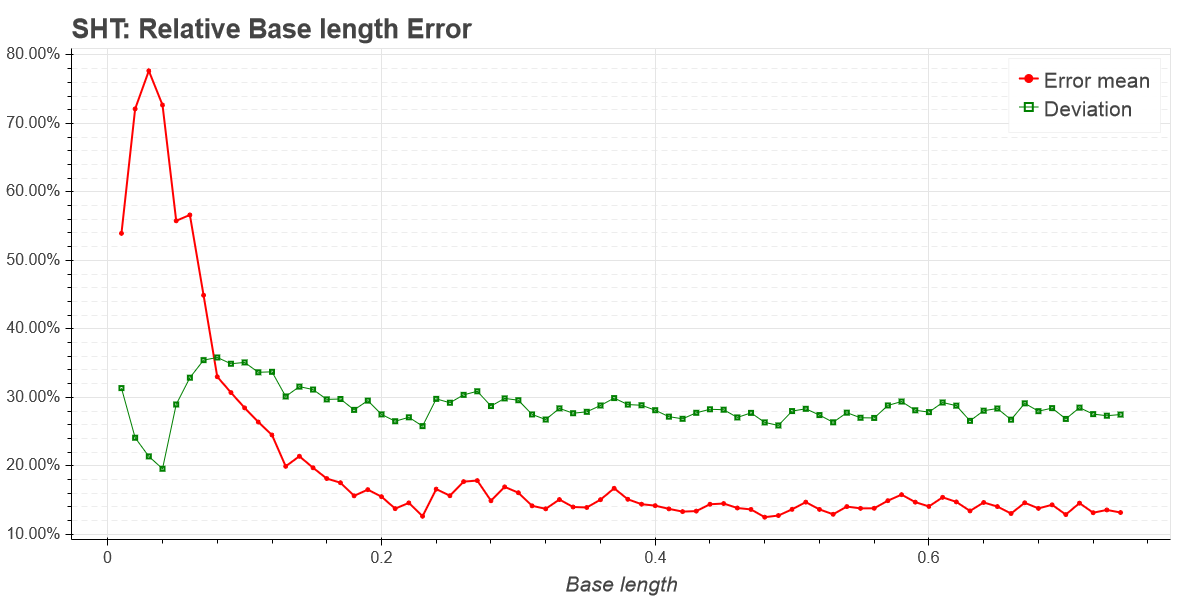
\includegraphics[width=0.9\textwidth]{figures/plots/sht_relative_base_length_error.png}
	\caption{Relative base length error with respect to quad size, using the SHT method}
	\label{fig:shtRelBaseErr}
\end{figure}

Figure \figref{shtRelCoordErr} shows the average relative coordinate error of the algorithm.
It is much larger than that of the LSD quad detector.
The error never goes below $15\%$, not even for large quads.
As stated above, the detector in it's current state is not recommended to be used on quads with a scale factor less than $0.2$.
At that scale, the coordinate error is $20\%$, which makes it's usefulness even more questionable.
\begin{figure}[ht]
	\centering
	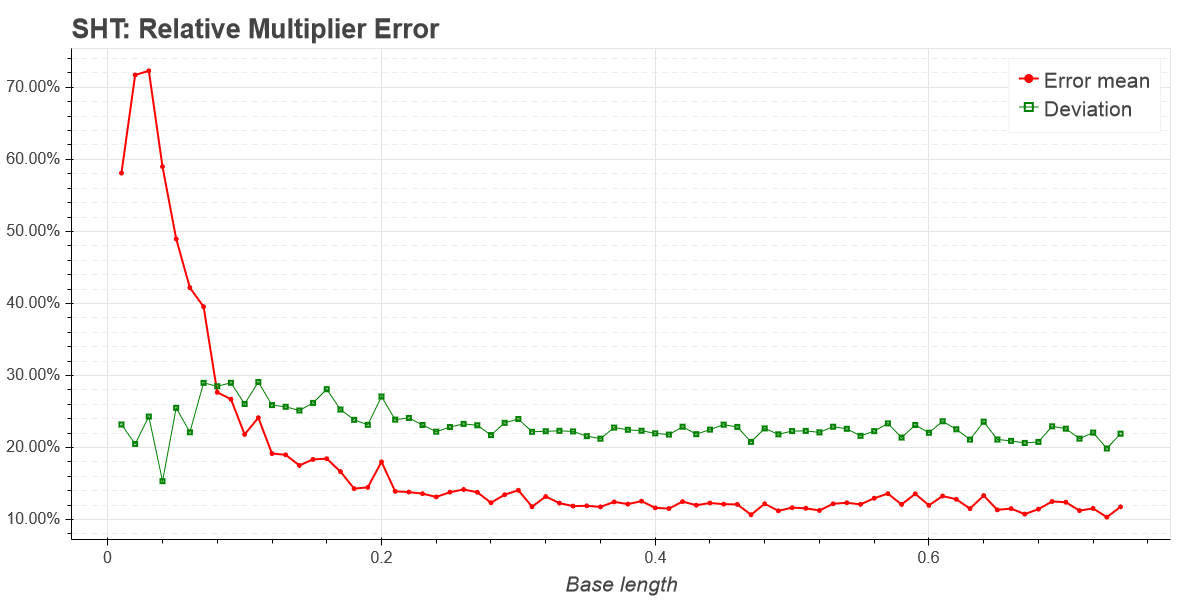
\includegraphics[width=0.9\textwidth]{figures/plots/sht_relative_multiplier_error.png}
	\caption{Relative multiplier error with respect to quad size, using the SHT method}
	\label{fig:shtRelMulErr}
\end{figure}

The error is distributed almost evenly between the quad parameters.
The base length and the multipliers have on average $15\%$ relative error in their optimal ranges.
The angle error shows a somewhat better picture, with it's $10\%$ minimal error.
The deviation is around $20\%$ for all of them.
The orientation is also the most accurately measurable parameter with this algorithm.
As figure \figref{shtRelOrientErr} shows, the relative error of the orientation stays below $10\%$ for the entire length range.
It's minimum is $2\%$, with $10\%$ deviation.
\begin{figure}[ht]
	\centering
	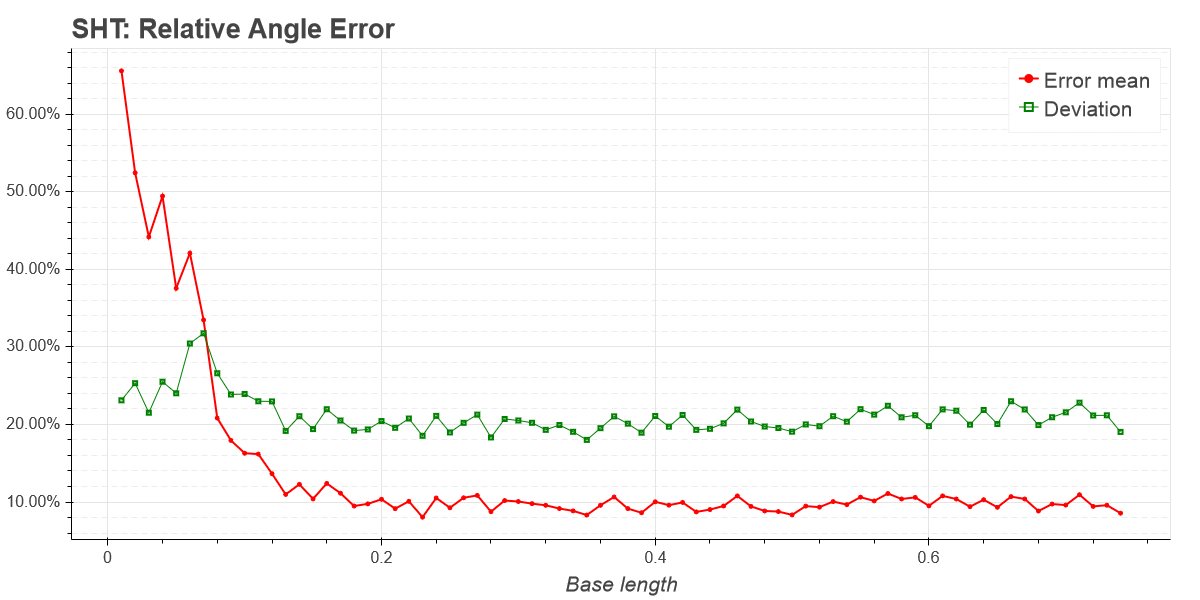
\includegraphics[width=0.9\textwidth]{figures/plots/sht_relative_angle_error.png}
	\caption{Relative angle error with respect to quad size, using the SHT method}
	\label{fig:shtRelAngleErr}
\end{figure}

There are many possibilities to further develop and refine this algorithm to provide much better results.
For example, the gradient information could be used to better detect lines, or a Least Squares approximation could be used to fit a line to the pixels marked as inliers to the line.
However, all this is true for the algorithm which uses the probabilistic Hough transform, which much better results.
Thus, further development of this algorithm is not recommended, nor will it be used further in the project.
\begin{figure}[ht]
	\centering
	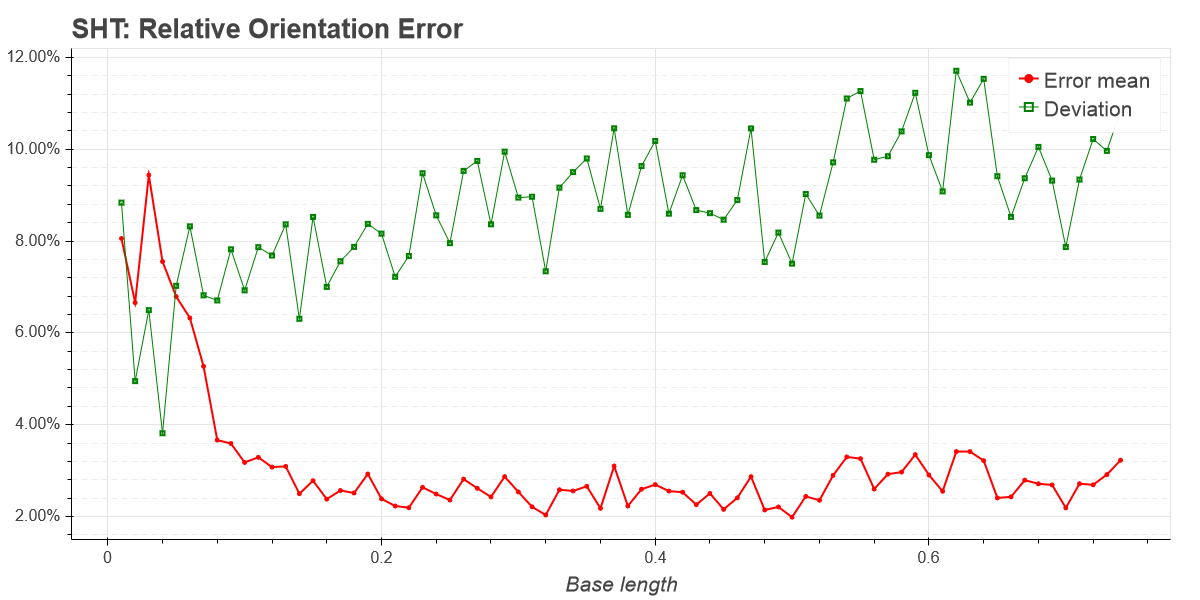
\includegraphics[width=0.9\textwidth]{figures/plots/sht_relative_orientation_error.png}
	\caption{Relative orientation error with respect to quad size, using the SHT method}
	\label{fig:shtRelOrientErr}
\end{figure}

%-----------------------------------------------------------------------------------------------
\clearpage\subsection{PHT Quad Detector results}
%-----------------------------------------------------------------------------------------------

In this section the performance of the probabilistic Hough transform-based quad detector will be evaluated.
The inner workings of the detector are very similar to the previously described SHT-based one.
\begin{figure}[ht]
	\centering
	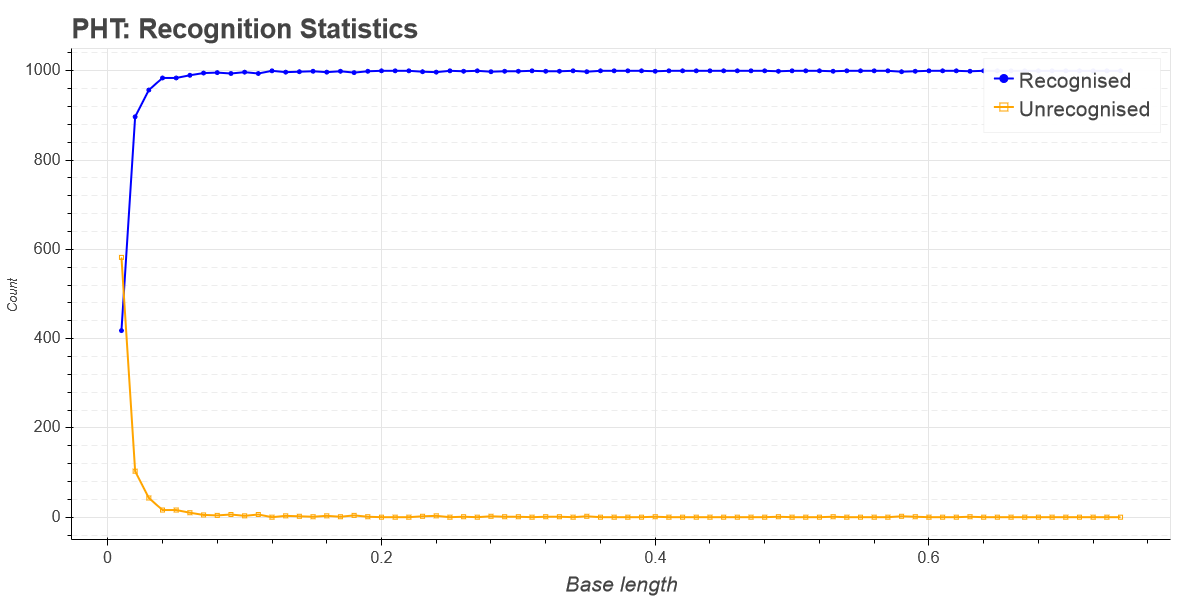
\includegraphics[width=0.9\textwidth]{figures/plots/pht_rec_unrec_count.png}
	\caption{Recognised and unrecognised quads with respect to quad size, using the PHT method}
	\label{fig:phtRecCnt}
\end{figure}
Nonetheless, this method is shows both better performance and requires less computation.
It was stated in the theoretical overview of the PHT that reducing the clatter in the accumulator improves the line detection results considerably.
Figure \figref{phtRecCnt} confirms this.
Opposed to SHT, the PHT based method detects even the smallest quads used for experimentation.
This detector proved to be the best consistently detecting a quad, although it's accuracy is not unparalleled.

\begin{figure}[ht]
	\centering
	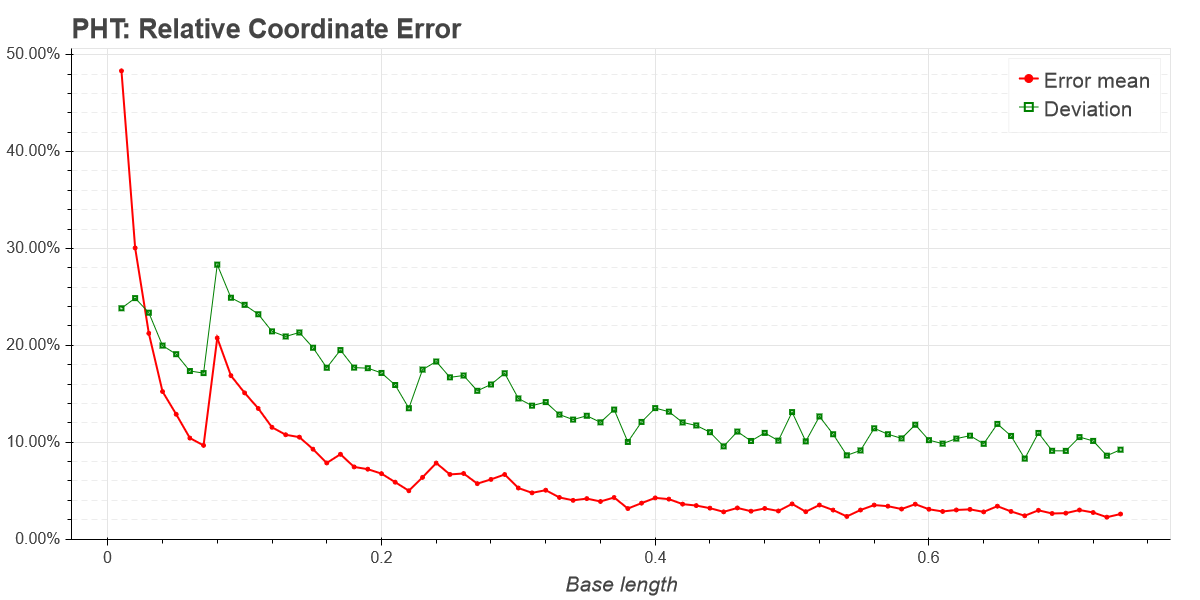
\includegraphics[width=0.9\textwidth]{figures/plots/pht_relative_coordinate_error.png}
	\caption{Relative coordinate error with respect to quad size, using the PHT method}
	\label{fig:phtRelCoordErr}
\end{figure}
The overall accuracy (that is, average relative error in corner the corner coordinates) is shown in figure \figref{phtRelCoordErr}.
Up from $0.1$ scale factor the error stays well below $20\%$, for most sizes (up from $0.2$) below $10\%$.
The minimum error is about $2\%$.
Note that the LSD detector in it's optimal range outperforms this, especially if the deviation is examined.

\begin{figure}[ht]
	\centering
	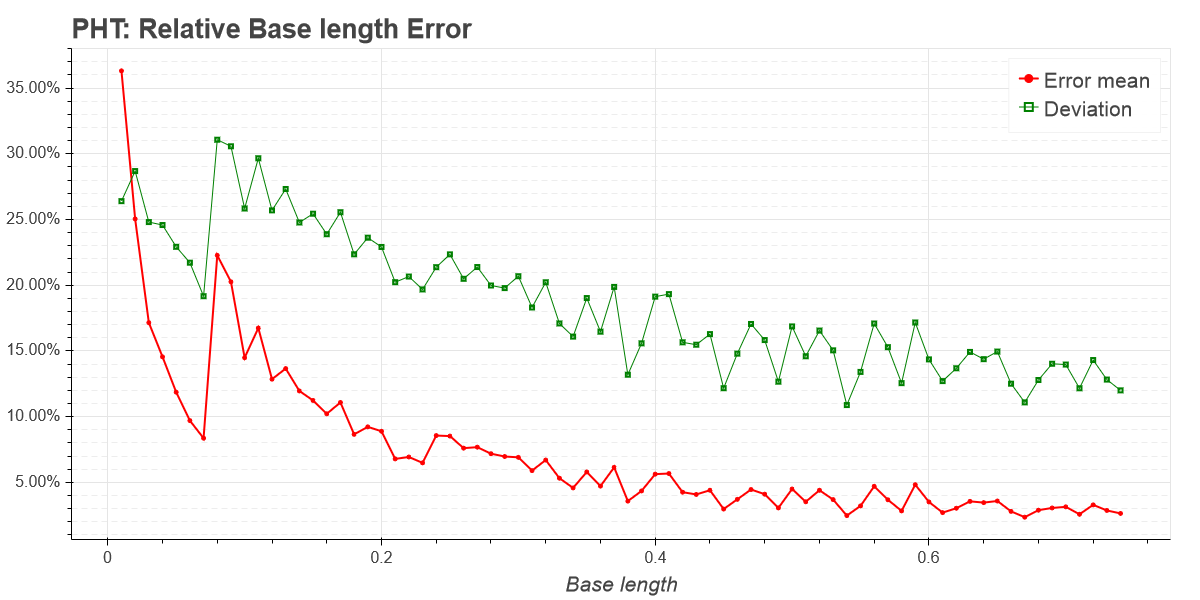
\includegraphics[width=0.9\textwidth]{figures/plots/pht_relative_base_length_error.png}
	\caption{Relative base length error with respect to quad size, using the PHT method}
	\label{fig:phtRelBaseErr}
\end{figure}
The error distribution between the quad parameters follows that of the SHT, only the magnitudes are much smaller.
The base length (figure \figref{phtRelBaseErr}), the side multipliers (figure \figref{phtRelMulErr}), and the angle error (figure \figref{phtRelAngleErr}) are in the same range.
For most sizes the error are below $10\%$, for large quads reaching their minimum of $2\%$.
Their deviation also follows the same trend, declining from $20\%$ to $10\%$.

\begin{figure}[ht]
	\centering
	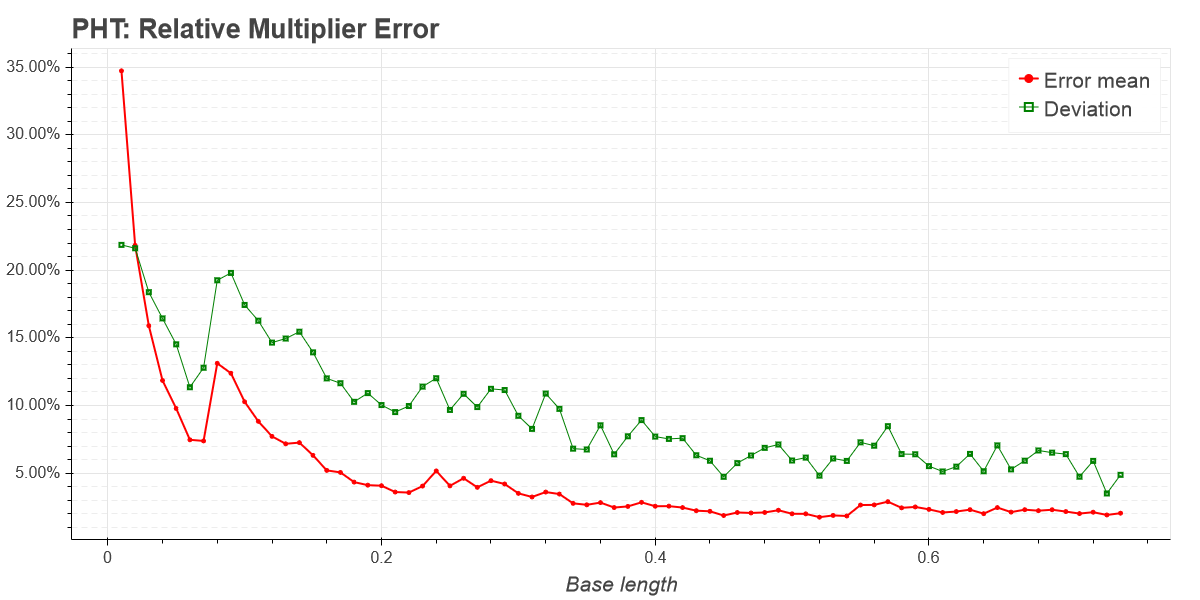
\includegraphics[width=0.9\textwidth]{figures/plots/pht_relative_multiplier_error.png}
	\caption{Relative multiplier error with respect to quad size, using the PHT method}
	\label{fig:phtRelMulErr}
\end{figure}
As for the orientation, similarly to the other detectors, it is the most accurately measurable quad parameter.
It is always measured within $4\%$ error margin, but for most sizes, within $2\%$.
The reason for this is was explained at the LSD detector: it depends only on the angle of the largest feature of the quad.
The error function is shown at figure \figref{phtRelOrientErr}.

This method significantly outperforms the SHT quad detector.
The two methods share most of the auxiliary logic between them.
They share the heuristics for the Hough parameter calculation (they differ in a scale factor for the threshold, as the PHT works with much less points), the segment matching, and most other functions as well.
This significant difference in performance is mainly due to the underlying transformation method.
\begin{figure}[ht]
	\centering
	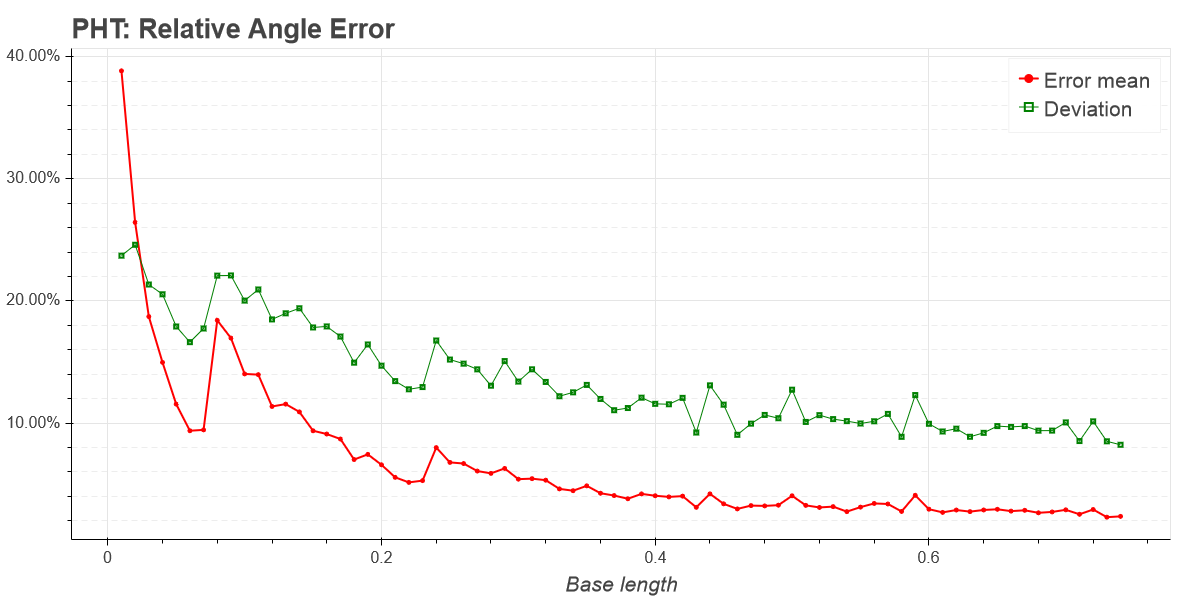
\includegraphics[width=0.9\textwidth]{figures/plots/pht_relative_angle_error.png}
	\caption{Relative angle error with respect to quad size, using the PHT method}
	\label{fig:phtRelAngleErr}
\end{figure}

If we look at the possible refinements of the algorithm, there is plenty.
Some have already been mentioned in the previous section, with the SHT algorithm.
Better parameter tuning is possible.
The skeletoning process which provides the input to the PHT algorithm also can be improved.
Incorporating the image gradient information in the transform would also significantly improve the results.
\begin{figure}[ht]
	\centering
	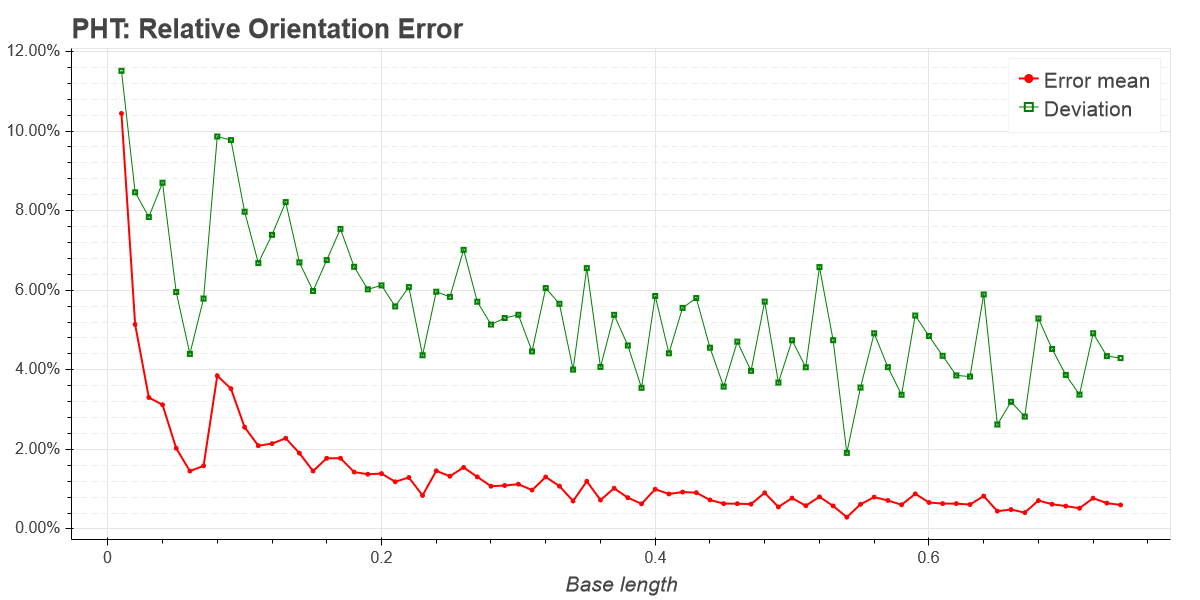
\includegraphics[width=0.9\textwidth]{figures/plots/pht_relative_orientation_error.png}
	\caption{Relative orientation error with respect to quad size, using the PHT method}
	\label{fig:phtRelOrientErr}
\end{figure}

%-----------------------------------------------------------------------------------------------
\clearpage\subsection{Corner Quad Detector results}
%-----------------------------------------------------------------------------------------------

The final quad detection method, contrary to the so far analysed ones, uses corner detection.
It shares the issue of tunable parameters with the Hough transformation based methods.
Below is the performance evaluation of the corner detection based quad detector.

As with the rest of the detectors, this one is a prototype, too.
This means there are multiple ways to improve it, but it is suitable for some preliminary experiments.

\begin{figure}[ht]
	\centering
	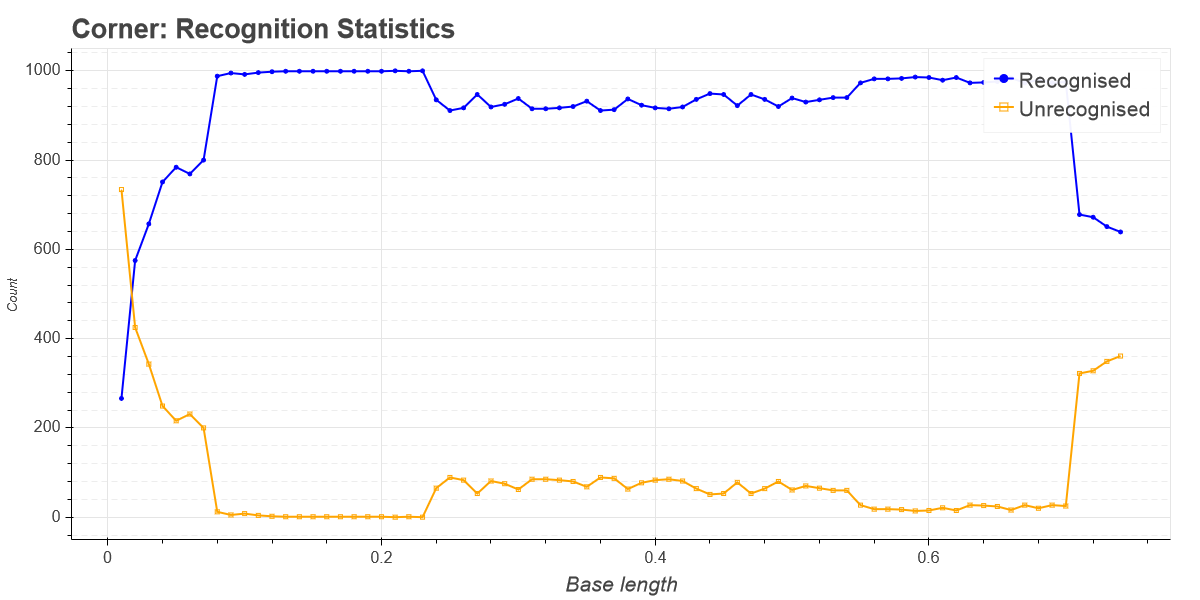
\includegraphics[width=0.9\textwidth]{figures/plots/corner_rec_unrec_count.png}
	\caption{Recognised and unrecognised quads with respect to quad size, using the Corner method}
	\label{fig:cornerRecCnt}
\end{figure}
Figure \figref{cornerRecCnt} shows the detection statistics of the detector.
Aside the really small quads, this method has potential to detect with remarkably good ratio.
There are 2 regions where almost all quads were detected.
However, in the middle size range, about $10\%$ of the quads were lost.
This is due to the rendering process and the lack of optimisation in the detection algorithm.
\begin{figure}[ht]
	\centering
	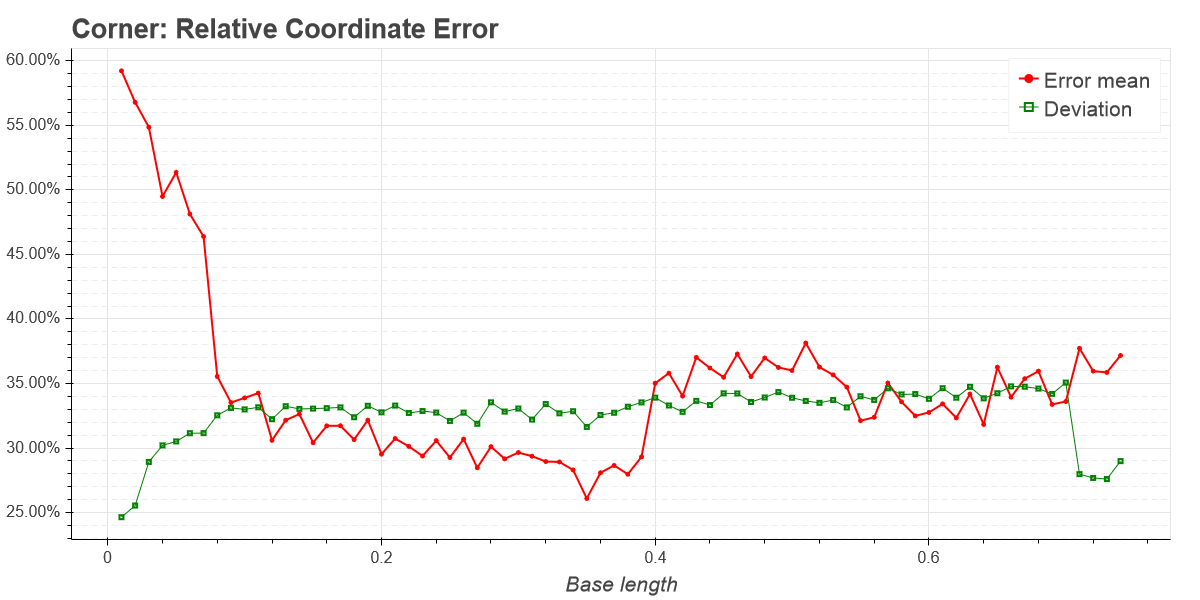
\includegraphics[width=0.9\textwidth]{figures/plots/corner_relative_coordinate_error.png}
	\caption{Relative coordinate error with respect to quad size, using the Corner method}
	\label{fig:cornerRelCoordErr}
\end{figure}
The parameters of the corner detector also need tuning to detect features on different scales.
In the middle region, the corners simply were too "round" to be detected.
This can be avoided with scaling of the image, or tweaking the detector parameters.

The same scaling issue can be observed on the error graphs as well.
These will not be considered in the error analysis, as they could be eliminated.
Only the optimal size range will be analysed.
\begin{figure}[ht]
	\centering
	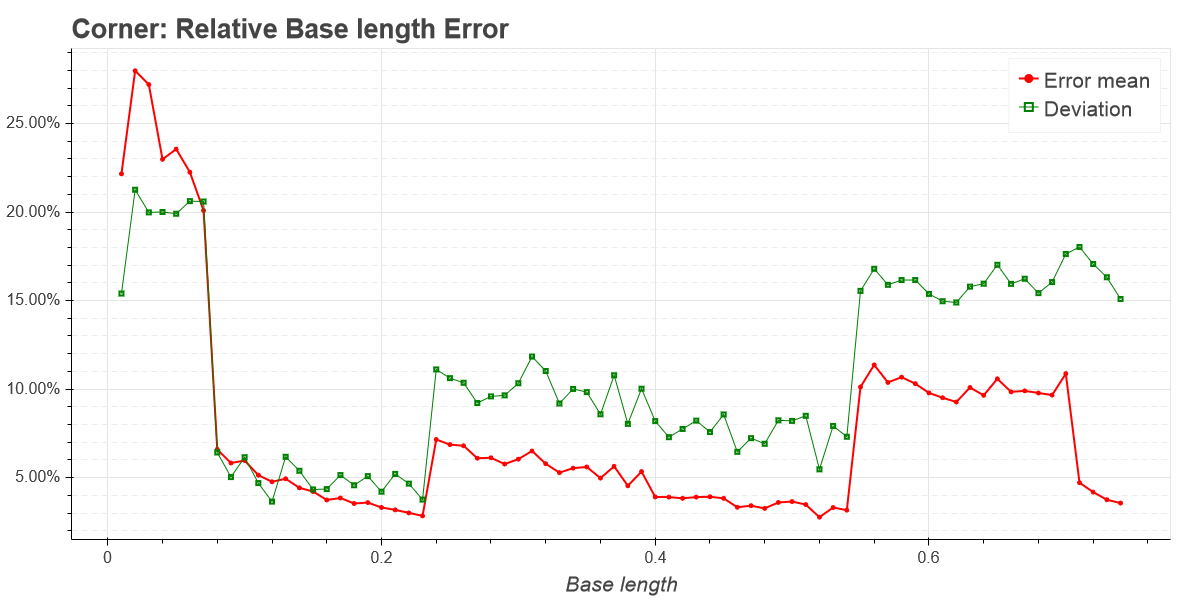
\includegraphics[width=0.9\textwidth]{figures/plots/corner_relative_base_length_error.png}
	\caption{Relative base length error with respect to quad size, using the Corner method}
	\label{fig:cornerRelBaseErr}
\end{figure}

The error in the corner positions is shown in figure \figref{cornerRelCoordErr}.
The magnitude is quite large, comparable to the one produced by the SHT-based method.
The reason for this is that the corner detector finds the outer, inner, or both corners os the \textit{edge} of the line, which can be quite far from the centre, depending on the quad angle and the viewpoint.
This could be somewhat compensated by using a skeleton, but finding an optimal algorithm for it is problematic.
\begin{figure}[ht]
	\centering
	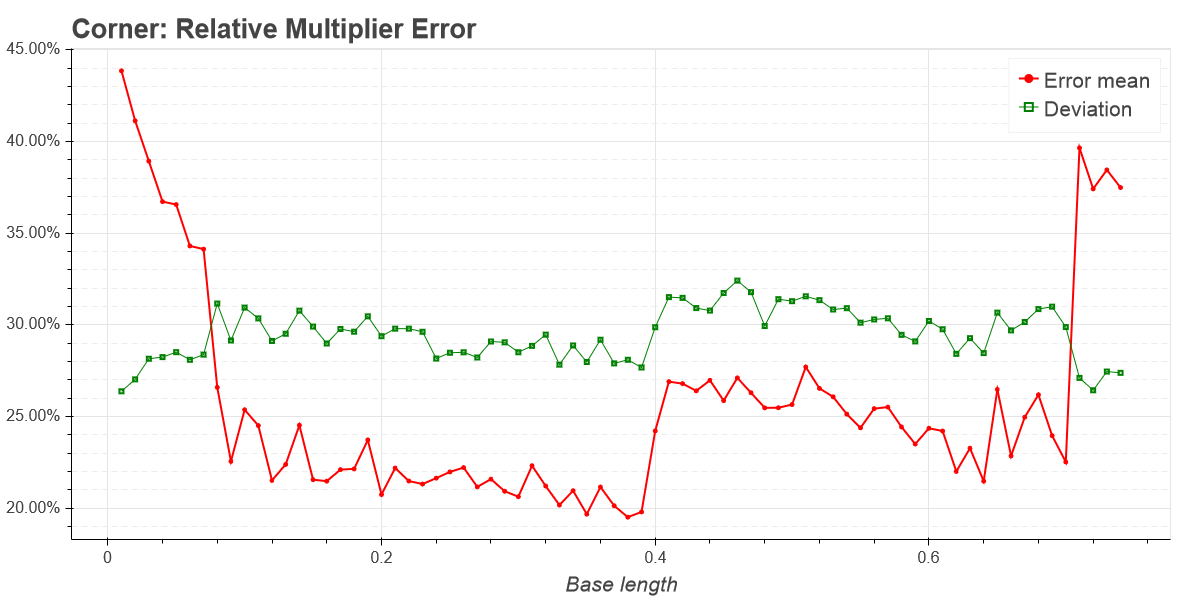
\includegraphics[width=0.9\textwidth]{figures/plots/corner_relative_multiplier_error.png}
	\caption{Relative multiplier error with respect to quad size, using the Corner method}
	\label{fig:cornerRelMulErr}
\end{figure}

The error of the base length detection is within reasonable limits, but it is far from being outstanding.
In it's optimal region, a $5\%$ error was achieved.
The orientation is also detected accurately enough.
The multipliers and the angle parameters on the other hand, carry quite a lot of error.
Their $30\%$ average value is far from usable, and is outperformed by the other algorithms.
\begin{figure}[ht]
	\centering
	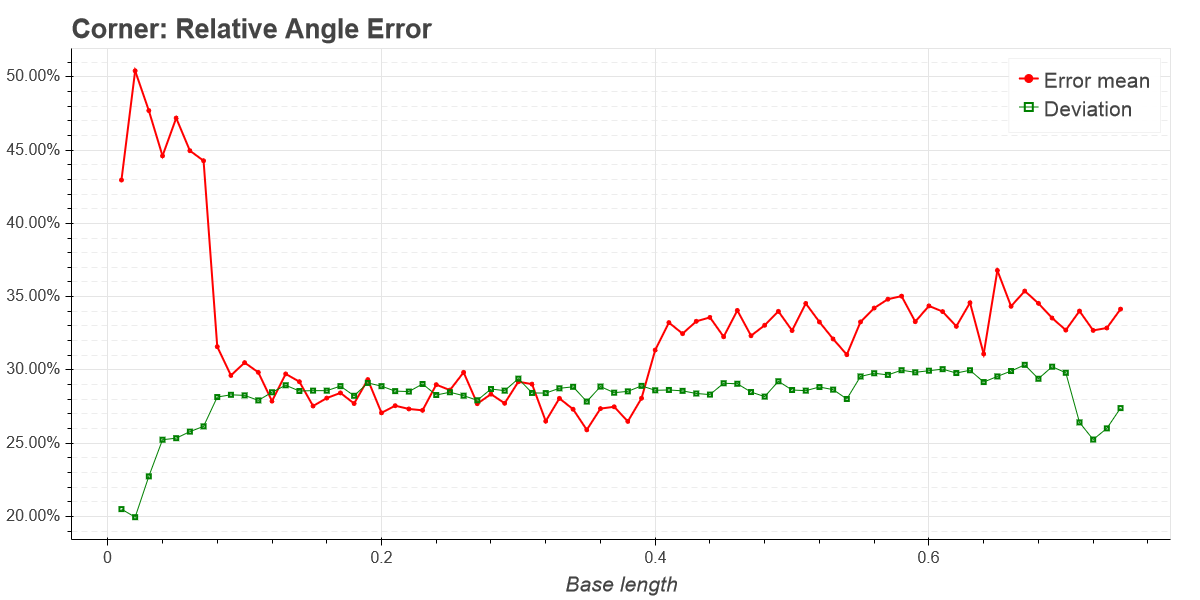
\includegraphics[width=0.9\textwidth]{figures/plots/corner_relative_angle_error.png}
	\caption{Relative angle error with respect to quad size, using the Corner method}
	\label{fig:cornerRelAngleErr}
\end{figure}

Based on these results, the application of corner detection is discouraged for this purpose.
As for the other algorithms, there are plenty opportunities for improvement, but the other solutions offer better performance overall.
Line segment detection seems a more intuitive solution for this problem, and, as expected, produced better results.
\begin{figure}[ht]
	\centering
	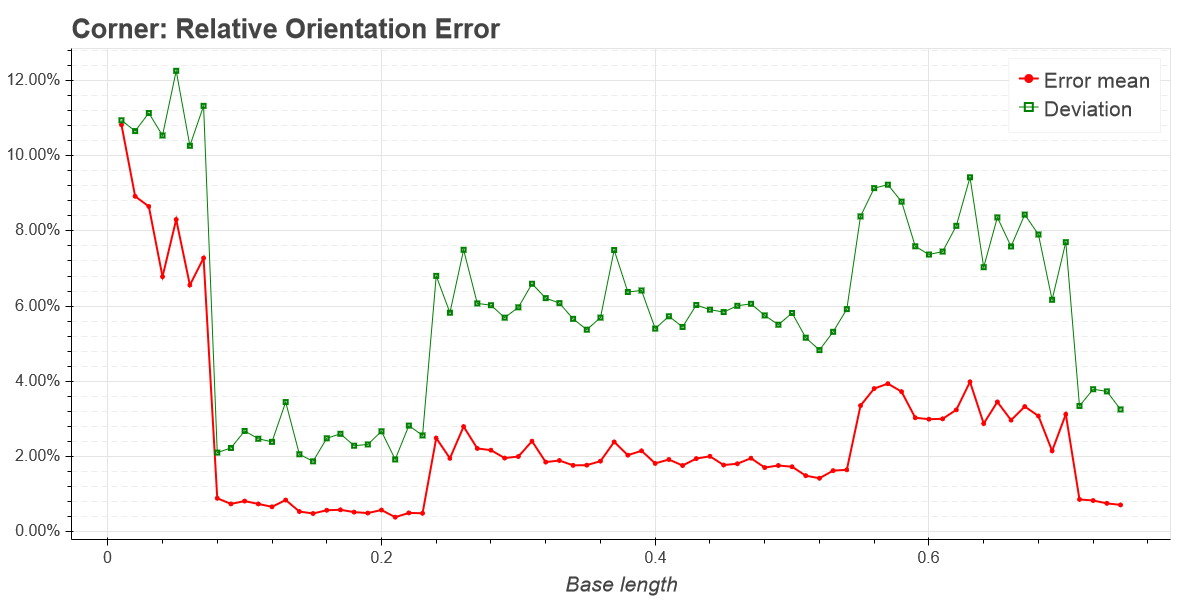
\includegraphics[width=0.9\textwidth]{figures/plots/corner_relative_orientation_error.png}
	\caption{Relative orientation error with respect to quad size, using the Corner method}
	\label{fig:cornerRelOrientErr}
\end{figure}

%-----------------------------------------------------------------------------------------------
\subsection{Summary}
%-----------------------------------------------------------------------------------------------

So far the performance of the quad detectors have been evaluated individually.
Now they will be compared against each other in order to select the most suitable one.
In this overall comparison the error distribution will not regarded, only the detection accuracy will be checked.
For this purpose the relative average coordinate error (defined by \eqref{errRelAvgCoord}) and the relative distance in the parameter space (defined by \eqref{errQuadSpaceDistRel}) will be used.

\begin{figure}[ht]
	\centering
	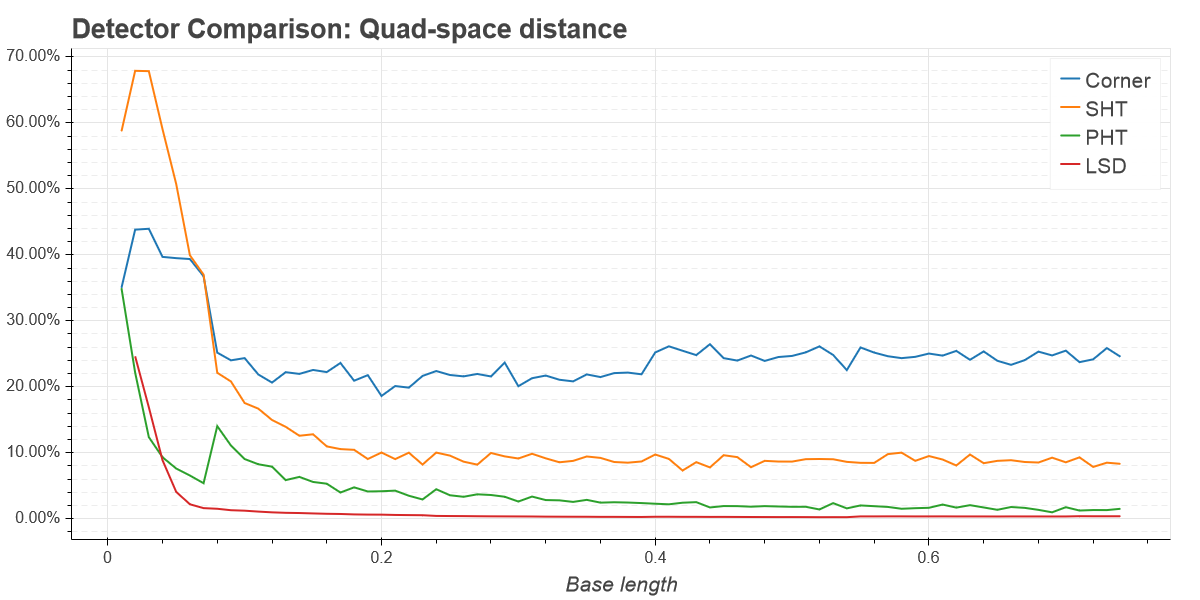
\includegraphics[width=0.9\textwidth]{figures/plots/detector_comp_quad_param_space.png}
	\caption{Detector comparison based on relative distance in parameter space}
	\label{fig:detCmpQSpace}
\end{figure}
Figure \figref{detCmpQSpace} shows a summary of detector performance based on distance in the parameter space.
As already mentioned, the corner detection based method is not recommended.
It has the greatest error magnitude out of the benchmarked algorithms.
With error rates greater than $20\%$, the usability of the estimated pose is questionable at best.

The second most error-prone detection method is the one based on the standard Hough transform.
At it's peak performance it works within a $10\%$ error margin.
Although much better than the corner detection based method, this level of accuracy is still not enough for robust pose estimation.
In terms of computational efficiency, the SHT is more expensive than the PHT or LSD.
As seen on the figure, the SHT also requires larger quads to provide acceptable error magnitude.

The second most promising algorithm turned out to be the probabilistic Hough transform.
It is a computationally efficient method which also provides reasonably accurate results.
For larger quads it performs nearly as well as the LSD based algorithm.
It may very well be possible to further refine the detection accuracy.

\begin{figure}[ht]
	\centering
	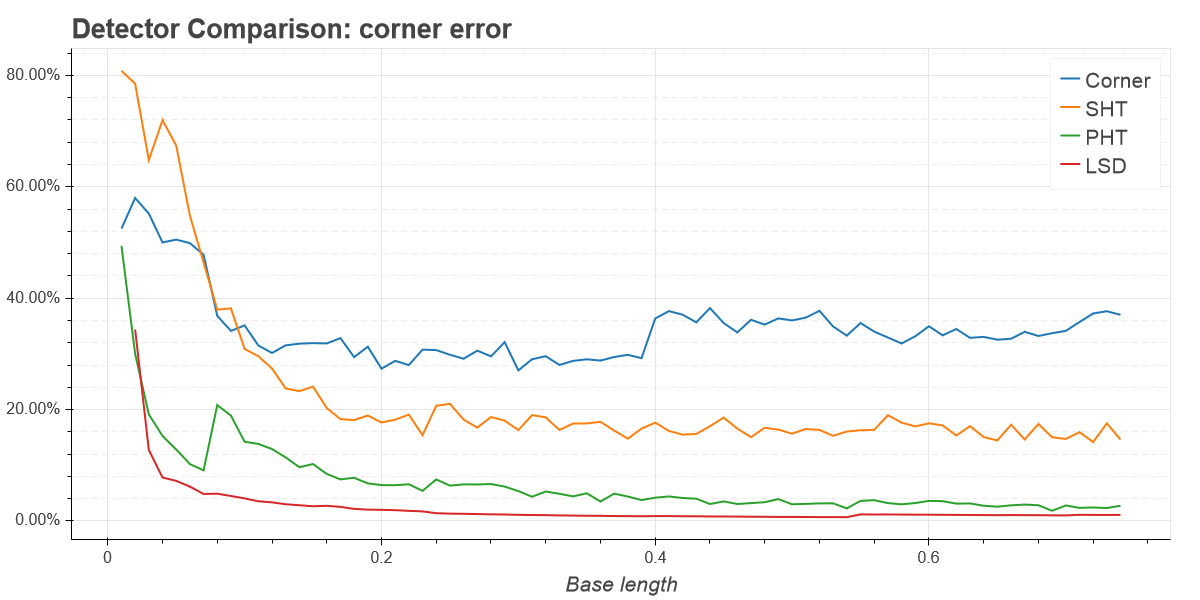
\includegraphics[width=0.9\textwidth]{figures/plots/detector_comp_corner_error.png}
	\caption{Detector comparison based on relative distance in parameter space}
	\label{fig:detCmpCorner}
\end{figure}
The clear winner is the LSD-based quad detector.
It clearly outperforms the other algorithms both in the parameter space distance and the relative corner error (figure \figref{detCmpCorner}).
It works reasonably well for small quads, has error magnitude as low as $1\%$ and the line detection routine runs in linear time.
Even if the PHT based detector comes close to it's accuracy, if the standard deviation of the error is also considered, the LSD is much more accurate.

Based on the individual and comparative tests, the following results have been found.
The corner detection based detector has too large error margins.
Even though run times were not measured in this test, it was also slower than the others.
The standard Hough transform based solution is somewhat better, and possibly could still be improved, but it is not recommended.
The PHT based detector outperforms it in every aspect, and since they are based on the same algorithm, it is recommended to focus on the PHT based variant.
It also performed well overall, with accuracy comparable to the LSD detector.
The PHT detector is recommended for further study or improvement.
The LSD detector proved to be the best in every situation examined in this experiment.
Due to it's accuracy and robustness, and also computational efficiency\footnote{Although this was not measured, the LSD algorithm runs in linear time, and the additional logic does not add much complexity} it is recommended to use it for quad detection in the further parts of this project.
